\chapter{Symulacje}

\section{Wprowadzenie}
W celu zasymulowania układu odwróconego wahadła i regulatora wykorzystano środowisko \textit{Matlab} \cite{matlab}. Metoda symulacji została oparta o pomysł przedstawiony przez S. L. Brunton'a \cite{Brun17}. Zmianą uległy równania na prędkości i przyspieszenia wahadła oraz sposób regulacji.

\section{Realizacja}
Oryginalnie do sterowania został wykorzystany regulator liniowo-kwadratowy -- LQR, który został  zastąpiony przez regulator propocjonalno-całkująco-różniczkujący -- PID. Projekt składa się z 4 plików:
\begin{itemize}
    \item simpend.m \ref{fig:simpend}
    \item drawpend.m \ref{fig:drawpend}
    \item cartpend.m \ref{fig:cartpend}
    \item mypid.m \ref{fig:mypid}
\end{itemize}
Plik \texttt{simpend.m} to plik uruchamiający cała symulację, gdzie możemy zmienić dane modelu czy nastawy regulatora. Pozostałe pliki zawierają definicje funkcji o tych samych nazwach. Funkcja \texttt{drawpend} jest odpowiedzialna za przedstawienie symulacji w sposób graficzny, rysuje wózek i wahadło w odpowiednim położeniu, jak na przykładowym rysunku \ref{fig:sim}.
\begin{figure}
    \centering
    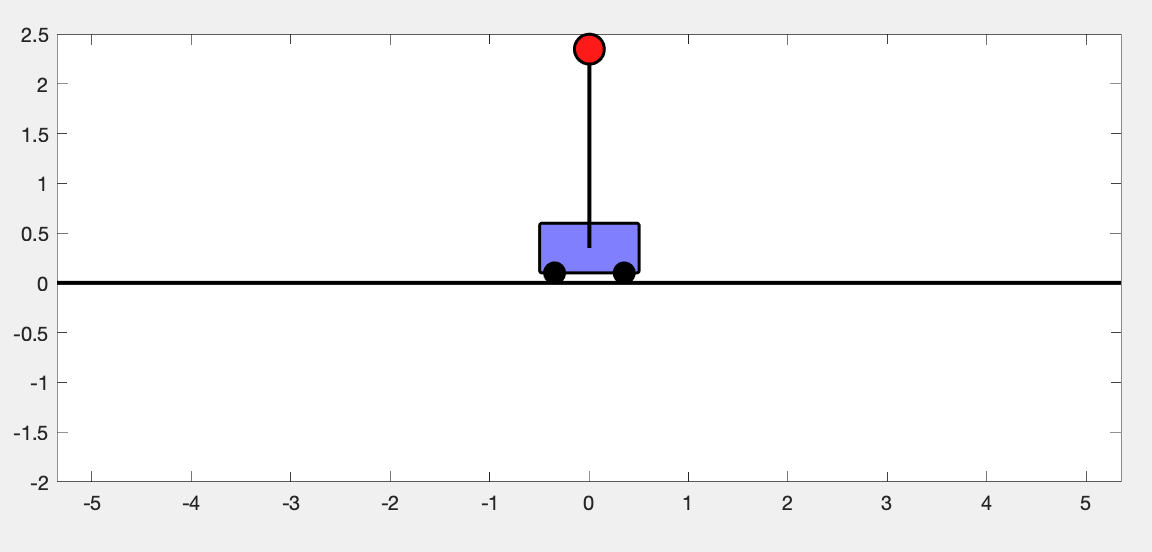
\includegraphics[scale=0.7]{praca_dyplomowa/figures/simulation.png}
    \caption{Animacja symulacji}
    \label{fig:sim}
\end{figure}
Funkcja \texttt{cartpend}, zawiera równania opisujące prędkość i przyspieszenie wahadła w zależności od czasu i danych wcześniejszych. Funkcja ta jest wykorzystywana przez wbudowaną funkcję \textit{ode45}, która rozwiązuje równania różniczkowe. Ostatnia funkcja to dyskretny regulator PID, która zwraca siłę, jaka powinna zostać przyłożona do wózka, aby utrzymać pręt w pozycji pionowej. 

Korzystając z równań dynamiki \ref{rDyna} można wyprowadzić wzory na prędkości i przyspieszenia liniowe i kątowe przez rozwiązanie układu równań.
\begin{equation}
    \begin{cases}
    (M+m)\ddot{x}+mL\ddot{\Theta}\cos{\Theta}-mL\dot{\Theta}^2\sin{\Theta}=F-T, \qquad T=f\dot{x}\\
    ml\ddot{x}\cos{\Theta}+mL^2\ddot{\Theta}-mgL\sin{\Theta} \Rightarrow \ddot{\Theta}=\frac{g\sin{\Theta}-\ddot{x}\cos{\Theta}}{L}
    \end{cases}
\end{equation}
\newline
\begin{equation}
    \begin{cases}
    (M+m)\ddot{x}+mg\sin{\Theta}\cos{\Theta}-m\ddot{x}\cos^2{\Theta}-mL\dot{\Theta}^2\sin{\Theta}=F-f\dot{x} \\ \\
    \ddot{\Theta}=\frac{g\sin{\Theta}-\ddot{x}\cos{\Theta}}{L}
    \end{cases}
\end{equation}
\newline
\begin{equation}
    \begin{cases}
    \ddot{x}(M+m-m\cos^2{\Theta})=mL\dot{\Theta}^2\sin{\Theta}-mg\sin{\Theta}\cos{\Theta}+F-f\dot{x} \\ \\
    \ddot{\Theta}=\frac{g\sin{\Theta}-\ddot{x}\cos{\Theta}}{L}
    \end{cases}
\end{equation}
\newline
\begin{equation}
    \begin{cases}
    \ddot{x}=\frac{mL\dot{\Theta}^2\sin{\Theta}-mg\sin{\Theta}\cos{\Theta}+F-f\dot{x}}{M+m-m\cos^2{\Theta}} \\ \\ \ddot{\Theta}=\frac{g\sin{\Theta}-\ddot{x}\cos{\Theta}}{L}
    \end{cases}
\end{equation}
\newline
\begin{equation}
    \begin{cases}
    \ddot{x}=\frac{mL\dot{\Theta}^2\sin{\Theta}-mg\sin{\Theta}\cos{\Theta}+F-f\dot{x}}{M+m-m\cos^2{\Theta}} \\ \\
    \ddot{\Theta}=\frac{mL\dot{\Theta}^2\sin{\Theta}\cos{\Theta}-(M+m)g\sin{\Theta}+F\cos{\Theta}-f\dot{x}\cos{\Theta}}{L(M+m-m\cos^2{\Theta})},
    \end{cases}
    \label{rowRuch}
\end{equation}
gdzie \textit{f} to współczynnik tarcia wózka.

\section{Sterowalność}

Linearyzacja równań \ref{rowRuch} pozwoli na zapis w formie równania macierzowego:
\begin{equation}
    \dot{x}(t)=Ax(t)+Bu(t)
\end{equation}
Zlinearyzowania można dokonać wokół punktów równowagi, czyli dla kąta wychylenia 0 lub \(\pi\). Z uwagi na założenie, że wahadło ma być skierowane do góry, istotniejszy jest kat odchylenia równy 0. Funkcje trygonometryczne przyjmą wartości:\(\sin{(\pi-\Theta)}=\sin{\Theta}\approx\Theta, \cos{(\pi-\Theta)}\approx\cos{\pi}=-1 \). Dzięki takiemu przybliżeniu, można zapisać równanie macierzowe:

\begin{equation}
\begin{bmatrix}
\dot{x}\\ 
\dot{v}\\ 
\dot{\Theta}\\ 
\dot{\omega}
\end{bmatrix}
=
\begin{bmatrix}
 0&  1&  0& 0\\ 
 0&  \frac{-d}{M}&  \frac{mg}{M}& 0\\ 
 0&  0&  0& 1\\ 
 0&  \frac{-d}{ML}&  \frac{-(M+m)g}{ML}& 0
\end{bmatrix}
\begin{bmatrix}
x\\ 
v\\ 
\Theta\\
\omega
\end{bmatrix}
+
\begin{bmatrix}
0\\ 
\frac{1}{M}\\ 
0\\ 
\frac{1}{ML}
\end{bmatrix}F
\end{equation}

Układ jest sterowalny wtedy i tylko wtedy, gdy macierz \textit{A} jest pełnego rzędu \cite{Mzyk05}. Rząd macierzy można obliczyć używając funkcji \textit{rank()} w środowisku \textit{Matlab} \cite{matlab}. W tym wypadku \textit{rank(A)=4}, a więc układ w otoczeniu punktu równowagi jest sterowalny. 